% !TEX root = ../main.tex
\pagebreak
\lecture{3}{2026-10-01}{Unternehmensethik}
\url{https://lms.uzh.ch/auth/RepositoryEntry/17910989063/CourseNode/102309852135373/path%3D~~VL%20III%20%2D%201%2E10%2E2026/0}
\section{Unternehmensethik}

\subsection{Aufgaben des Managements in einer Unternehmung} 

\subsection{Fall Nestle}
"Da Zutaten aus Weltmarkt gewonnen werden müssen, können Arbeitsbedingungen nicht sichergestellt werden". \footnote{Ist nicht die Absenz gerechte Arbeitsbedingungen, genau der Grund wieso solche Länder quelle von Rohstoffe sind. und wenn Unternhmen selbst die Politik beeinflüssen um ausbeutungs Bedingungen sic}

\subsection{Koordinationsinstrument}
\begin{itemize}
    \item Dezentrale Koordination
    \begin{itemize}
        \item Markt, Wettbewerb, Preissystem
    \end{itemize}
    \begin{itemize}
        \item Im Vergleich zur Planwirtschaft
    \end{itemize}
    \begin{itemize}
        \item Besserer Umgang mit dem Kalkulationsproblem (wohin investieren und wie viel)
        \item Kontrollproblem
        \item Gewinne sind nicht dafür da, Kapitalisten die Tasche zu füllen, sondern leiten Ressourcen in die "richtige" Richtung
    \end{itemize}
\end{itemize}

\subsection{Vertragsmodell: Unternehmung als ergänzendes Koordinationsinstrument}

\begin{itemize}
    \item Eigentumsrecht
    \begin{itemize}
        \item Produktionsmittel 
    \end{itemize}
    \item Staat schützt Eigentum, und Vertragsrecht, sichert die Bedingungen zur Funktion der kapitalistischen Marktwirtschaft
    \item Vertragsmodell: Einheit von Risiko und Gewinn bzw. Verlust
    \begin{itemize}
        \item Kapitaleigner tragen das Risiko und erhalten [darum] \textit{Residualeinkommen} bei Erfolg \footnote{Nur das finanzielle Risiko, das mit der Gesellschaftsform verbunden ist, das tatsächliche körperliche, psychische Lebensrisiko tragen arbeitenden Menschen}
    \end{itemize}
\end{itemize} 
\pagebreak
\subsection{Vertragsmodell: Grenzen}
Beruht auf unrealistischen Annahmen.
\begin{itemize}
    \item Trotz interner und externer Regelungen kann die reale Funktionsfáhigkeit des Preissystems nicht sichergestellt werden. \footnote{Idealismus: Es sieht die echte Funktionsweise als ein unabhängig existierendes Konzept.}
    \item 3 Problembereiche der kapitalistischen Marktwirtschaft
    \begin{itemize}
        \item Trennung von Eigentum und Entscheidungsmacht
        \item Vermachtungsprozesse im Wettbewerb
        \item Externe Effekte
    \end{itemize}
\end{itemize}

\subsubsection{Problematik: Trennung von Eigentum und Entscheidungs- bzw. Verfügungsgewalt}

\begin{itemize}
    \item Vertragsmodell stellt eine Einheit von Eigentümer und Entscheidungsgewalt auf Basis von Präferenzen dar.
    \item Heute aber Trennung von Eigentum und Entscheidungsgewalt, sodass:
    \begin{itemize}
        \item Kapitaleigentümer sind nur Aktionäre im Hintergrund \footnote{Thematisiert wird nicht Trennung des Eigentums von den Arbeitenden, also die die tatsächlich produzieren und als Klasse konsumieren, sondern das Problem wäre die interne Trennung von Aktionäre und Manager.}
        \item Professionelle Manager tragen Entscheidungen
    \end{itemize}
    \item Gründe
    \begin{itemize}
        \item Professionalisierung des Managements
        \item Inaktivität der Eigentümer
        \item "Vergesellschaftung der externen  oder Kosten und private Aneignung von Gewinne"
    \end{itemize}  
    \item Folgen
    \begin{itemize}
        \item Darum seien Entscheidungen gefällt, die nicht einer \textit{nachhaltigen Unternehmensentwicklung} entsprechen.
    \end{itemize}
\end{itemize}


\pagebreak
\subsubsection{Problematik: Vermachtungsprozesse}
Durch Macht können Akteure, ihre Interessen willkürlich gegen andere durchsetzen. 

\begin{itemize}
    \item ökonomisch (Oligopole Preisbildung)
    \item Politisch (Lobbying)
    \item Ressourcenbezogen (Monopol Zugang natürlichen Resourcen)
\end{itemize}

\subsubsection{Problematik: Externe Effekten}
\begin{definition}
    [Externen Effekte] Auswirkungen wirtschaftlicher Betätigung von Unternehmen oder Haushalten auf Dritte, die sich nicht über das Preisszstem vollständig repräsentieren lassen. Unvollständige Informationen in den Preisen. \footnote{Weil preise nur ausdruck von Wert sind oder Ausdruck gleicher gesellschatlichen Arbeitszeit}  
\end{definition}
\subsection{Zwischenfazit}

\textbf{Koordination über Markt allein nicht zureichend}

Korrekturversuch: \textit{Verständigungsorientierte Koordination} \footnote{Ist die naturwüchsige Koordination der gesellschaft freier Produzenten, das sollte, ihrer Meinung nach, in der Kapitalistischen gesellschaft implementiert werden, ohne dabei die Frage zu stellen, ob das überhaupt möglich ist. Scheitern der UNO, Völkerbund etc.} gegen die "Erfolgsorientierte Koordination"
\begin{itemize}
    \item Kommunikative Rationalität
    \item Interesse anderer Akteuren berücksichtigen
    \item Argumentative auseinandersetzung (nicht allein durch private Interessen) \footnote{basically Kategorische Imperativ für wirtschaft}
    \item Middleground finden weil kommunikation sehr viel zeit benötigt. 
\end{itemize}

\subsection{Legitimität}

\begin{definition}
    [Legitimität] generalisierte Einschätzung der Unternehmung durch ihre Bezugsgruppen. Wünsch von der Allgemeinheit als vertretbar, erwünscht, richtig, oder angemessen wahrgenommen zu werden.
\end{definition}
\pagebreak
\subsubsection{Die 3 Arten}

\begin{itemize}
    \item Kognitive
    \begin{itemize}
        \item Unbewusst/Irrational
        \item nicht hinterfragene soziale Normen
        \item Es ist einfach so, also akzeptieren wir's 
    \end{itemize}
    \item Pragmatische
    \begin{itemize}
        \item Vernünftig/rational
        \item Kosten-Nutzen Kalkulation
        \item Eigennutzen \footnote{'Kapitalismus ist Institution in der Alle profitieren' wäre so eine pragmatische Aussage. Stimmt so einfach nicht, wir sehen verlierer länder, gewinner Länder, arme und reiche innerhalb eines Landes" - Prof. Scherer }
    \end{itemize}
    \item Moralische 
    \begin{itemize}
        \item Normative bewertung der Unternehmung und ihrer Handlungen
        \item Beispiel Nestle \footnote{Möglichkeit nicht mehr aus dominierten Länder Palmöl kaufen weil soziale udn umweltliche folgen. }
    \end{itemize} 
\end{itemize}

\subsection{Stakeholder-Ansatz}

Totalität der Bezugsgruppen bei Entscheidungen berücksichtigen. Gegenstück des Shareholder-Ansatzes, das nur unmittelbare Kunden, Aktionäre, Eigentümer bevorzugt.

\subsubsection{Klassifikation der Stakeholden}
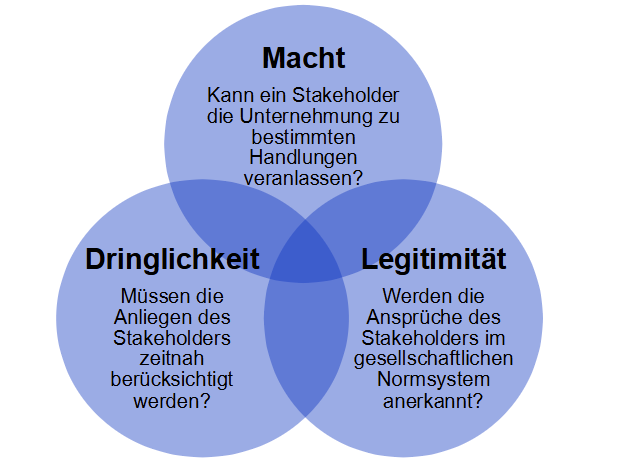
\includegraphics[width=\textwidth,height=0.7\textheight,keepaspectratio]{figures/Venn_Stakeholder.png}

\subsubsection{Materialitätsmatrix Néstlé}


\subsubsection{Bewertung Stakeholder-Ansatz}

\begin{itemize}
    \item erweitert erfolgsorientierung mt Verständigungsorientierte dimension
    \item Restriktion des Prinzips der Gewinnmaximierung
    \item Monologische Ausrichtung (Entscheidungen trotz noch aufseite der Internen manager \textbf{kein dialog})
    \item Interessen Stakeholder finden nur ANklang bei Schnittmenge mit Gewinnmaximierung \footnote{also nur Nice to have, keine grundlegende veränderung, wie Monarchischer Parlamentarismus}
\end{itemize}